\section{Test Strategy}
\label{sec:test_stra}

The validation has to demonstrate that the openETCS tool chain covers all the functionality. This test strategy will be divided in four sides, the building test, installation test, functional test and performance test:
\begin{itemize}
\item Building testing: The main objective is to check the correct building of the toolchain.
\item Installation test objective: The main objective will be to validate that the OpenETCS platform and the plugins, are correctly installed, and their interoperability is correctly working.
\item Functional test objective: The main objective will be validating that the user’s workflows are correctly created and to provide clear evidence that the platform performs as it should in every possible environment.
\item Performance testing: The main objective is to verify the performance of the tool chain.
\end{itemize}

\section{Test Items}
\label{sec:test_items}
\todo[color=yellow!20, inline]{IT: Brief introduction to the figure. Explanation about how it will grow -according to new feature requests and the
needs of openETCS participants-}


\begin{figure}[htbp]
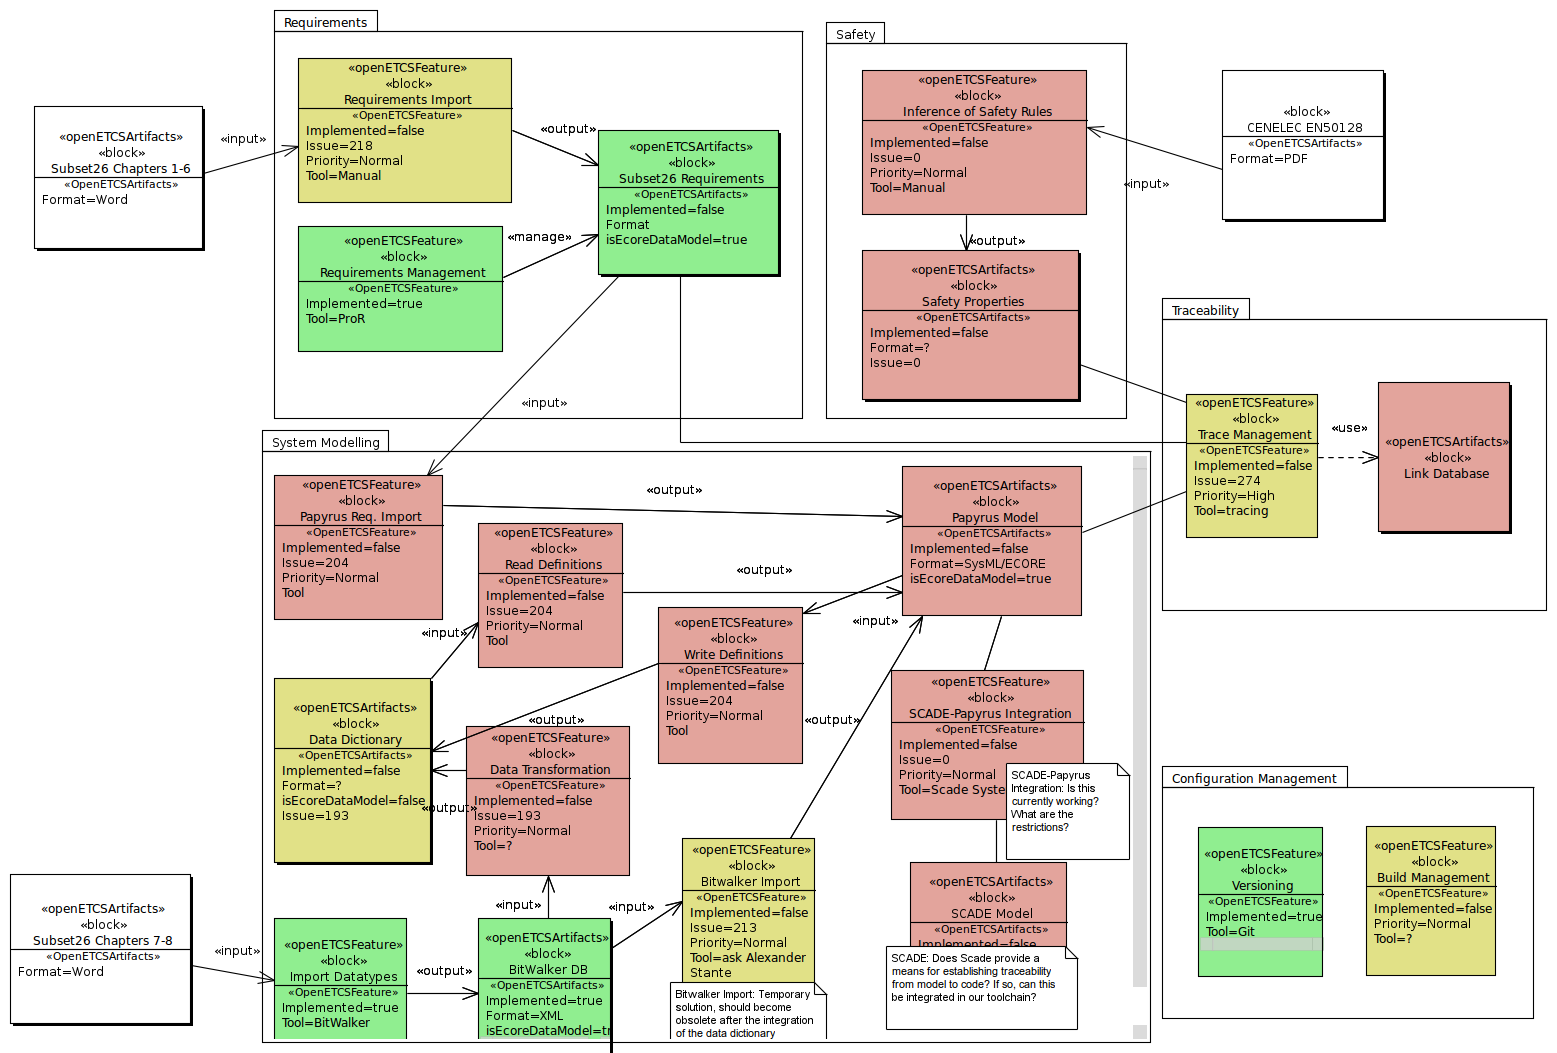
\includegraphics[width=\textwidth]{ToolChainmodel}
\caption{\label{fig:overview} Tool Chain overview (20.02.14) -- \\
  Green Block: Implemented \\
  Yellow Block: Work in Progress \\
  Red Block: Not started \\
  White Block: External Artifacts} 
\end{figure}

The features may be implemented by one or more tools and may also be implemented as plugins.

Currently, openETCS tool chain consists of the following components:
\begin{itemize}
\item Eclipse Kepler
\item Eclipse Modeling Tools
\item Eclipse Papyrus
\item Eclipse RMF
\item Eclipse EGit
\item openETCS documentation Plugin
\item openETCS DataDictionary Plugin
\item openETCS tracing Plugin
\end{itemize}

The plugins that are going to be part of the first release of the test plan will be:
\begin{itemize}
\item \textbf{Data Dictionary}: This plugin contains the data dictionary plugin which contains data structures, variables, messages, etc. from the ETCS System Requirements Specification (SRS). The plugin registers a UML model, which contains the information from the SRS. After registration, the UML model is available as a UML library.
\item \textbf{Tracing}: The Tracing Features allow the linking of *ProR Requirements* and *SysML Model Elements*. This is realized within the requirements model by using the internal links (SpecRelations) and requirements that act as proxies to the SysML Model element. Note that both, links and proxies, can be extended with additional attributes.
\item \textbf{Documentation}: The documentation plug-in generates Eclipse Help documentation (a hierarchy of HTML files) and PDF documentation from toolchain wiki pages saved as mediawiki.
\end{itemize}

\begin{center}
\begin{longtable}[H]{|p{6cm}|p{4cm}|p{4cm}|}\hline
\textbf{Test Items} & \textbf{Type of Test} & \textbf{Person in charge}\\\hline
\multirow{4}{*}{openETCS documentation Plugin} & Unit Testing & \\\cline{2-3} & Integration Testing & \\\cline{2-3} & Functional Testing & \\\cline{2-3} & Acceptance Testing & \\\hline
\multirow{4}{*}{openETCS DataDictionary Plugin} & Unit Testing & \\\cline{2-3} & Integration Testing & \\\cline{2-3} & Functional Testing & \\\cline{2-3} & Acceptance Testing & \\\hline
\multirow{4}{*}{openETCS tracing Plugin} & Unit Testing & \\\cline{2-3} & Integration Testing & \\\cline{2-3} & Functional Testing & \\\cline{2-3} & Acceptance Testing & \\\hline
\end{longtable}
\end{center}


\section{Features to be tested}
\label{sec:features_test}

\begin{center}
\begin{longtable}{|p{2cm}|p{8cm}|}\hline
%\centering
%\begin{tabular}{|p{2cm}|p{8cm}|}\hline
\multicolumn{2}{|c|}{ProR}\\\hline
1 & Check if the RMF documentation is on Eclipse Help\\\hline
2 & Check if is possible to import a ProR requirements model\\\hline
3 & Check if it is possible to import a SysML requirements model\\\hline
4 & Check if it is possible to create a link between ProR and SysML\\\hline
5 & Check if it is possible to add extended attributes to the created links\\\hline
6 & Check how are created the required type of data.\\\hline
7 & Check if it is possible to delete required type of data\\\hline
8 & Check the plugin configuration\\ \hline
9 & ... \\ \hline
\multicolumn{2}{|c|}{Documentation}\\\hline
1 & Check if the documentation is on the eclipse help\\\hline
2 & Check if the links are correct in Eclipse Help\\\hline
3 & Check if the links are correct in the github wiki pages\\\hline
4 & Check if the links are correct in the PDF file\\\hline
5 & ...\\ \hline
\multicolumn{2}{|c|}{Data Dictionary}\\\hline
1 & \\ \hline
%\end{tabular}
\end{longtable}
\end{center}


\section{Item Pass / Fail Criteria}
A test is considered passed when the results obtained are the expected results shown in the Test Case. If any of the expected results are not met, the test is considered failed.

\section{Test Environment}
The environments where is going to be tested the toolchain are based on different operating systems:
\begin{itemize}
\item Windows 64
\item Windows 32
\item Linux 64
\item Linux 32
\item MacOS 64
\item MacOS 32
\end{itemize}

To perform the testing activities of the toolchain the following tools will be used:

\begin{center}
\begin{longtable}{|p{2cm}|p{8cm}|}\hline
\textbf{Tool} & \textbf{Functionality}\\\hline
GitHub & Configuration Management tool. This tool will be used to maintain under control all the selected configuration items (code, documentation,...), their versions and historial.\\\hline
Issue Tracker & Tool for the Bug Management and Tracking. The errors found during testing activities will be reported in this tool\\\hline
Jenkis & Open source continuous integration tool. This tool will be used to execute Unit tests.\\\hline
Maven &  Build automation tool. This tool will be used to execute some integration tests.\\\hline
Eclipse & \\\hline
\end{longtable}
\end{center}


\section{Test Deliverables}
Throughout the tool chain testing process a set of documents is created in order to keep track of the activities:
\begin{itemize}
\item \textbf{Test Plans}: A master test plan and sub-test plans for each plugin or feature will be developed. These documents will contain information about the scope, approach, objectives, features to be tested, resources, tools and schedule of testing activities.  These documents must be prepared in accordance with the EN50128 Standard. A Test Plan Template is provided in Appendices \ref{ref:test_plan_template}
\item \textbf{Test Specifications}: This document will contain all the information about the tests. For each of them, the ID, name, description and the requirements which the cases validate will be included. In addition, each Test Case will include information about the Entry and Exit specification, a Description of the Event to be performed and other information such as type or Needs Test Environment for conducting the test. The Test Specification Template is provided in the Appendices \ref{ref:test_spec_template}
\item \textbf{Test Results Reports}: The results obtained after the Test Cases execution will be collected in a Summary Test Report. For each test performed their unique identifier, the date and time which has been successfully executed or not and whether it is passed or failed state shall be indicated. A Test Results Report Template is provided in the Apendices \ref{ref:test_result_template}. In case the tests are executed automatically by a tool that creates its own report, this will also be used as Test Result Report. An example of this last condition is the unit test result report which can be found in \href{https://openetcs.ci.cloudbees.com/job/openETCS-tycho/lastBuild/testReport/}{[Test Report folder]}.
\item \textbf{Test Data}: All necessary data identified for use in test shoud be under configuration management tool.
\item \textbf{Test Incident Report}:
\item \textbf{Test Logs}:
\end{itemize}

\section{Schedule}
The plan of tasks related to the activities of the toolchain tests is detailed below:
\begin{table}[htbp]
\centering
\begin{tabular}{|p{8cm}|p{3cm}|p{3cm}|}\hline
\textbf{Activity} & \textbf{Start Date} & \textbf{End Date}\\\hline
Test Plan Elaboration & 14/08/2014 & 05/09/2014 \\\hline
Test Plan Review & 08/09/2014 & 12/09/2014\\\hline
Test Plan Corrections & 15/09/2014 & 18/09/2014\\\hline
Test Plan Approval & 19/09/2014 & 19/09/2014\\\hline
\multicolumn{3}{|l|}{Test Cases Specifications}\\\hline
Documentation Plugin Test Cases Specifications & 01/09/2014 & 03/09/2014\\\hline
Tracing Plugin Test Cases Specifications & & \\\hline
Data Dictionary Plugin Test Cases Specifications & & \\\hline
\multicolumn{3}{|l|}{Test Cases Review}\\\hline
Documentation Plugin Test Cases Review & & \\\hline
Tracing Plugin Test Cases Review & & \\\hline
Data Dictionary Plugin Test Cases Review & & \\\hline
\multicolumn{3}{|l|}{Test Cases Execution}\\\hline
Documentation Plugin Test Cases Execution & & \\\hline
Tracing Plugin Test Cases Execution & & \\\hline
Documentation Plugin Test Cases Execution & & \\\hline
\multicolumn{3}{|l|}{Test Results Report}\\\hline
Documentation Plugin Test Results Report & & \\\hline
Tracing Plugin Test Results Report & & \\\hline
Data Dictionary Plugin Test Results Report & & \\\hline
\end{tabular}
\end{table}

\section{Responsabilities}
\begin{center}
\begin{longtable}[H]{|p{3cm}|p{8cm}|p{4cm}|}\hline
\textbf{Role} & \textbf{Responsabilities} & \textbf{Person in charge}\\\hline
WP7 Leader & \begin{itemize}
\item Review and approval of the toolchain testing strategy, approach, and plans
\item Review of testing results report and defects to determine the impact to overall tool chain and plugins  development and implementation schedule
\end{itemize}  
 & Michael Jastram\\\hline
Testing Manager & \begin{itemize}
\item Develop Test Strategy and Test Plan
\item Coordinate the development of testing deliverables
\item Review and approve testing deliverables
\item Monitor and report on the status of testing activities
\item Coordinate testing activities
\item Defect management
\end{itemize}  
 & \\\hline
SW Development Team & \begin{itemize}
\item Design Unit Test Cases
\item Execute Unit Test Cases
\item Review test cases and results for completeness
\end{itemize}  & Plugin or Feature Owner\\\hline
Tool chain Validation and Verification Team & \begin{itemize}
\item Design Test Cases
\item Execute Test Cases
\item Elaborate Test Reports
\end{itemize}
& \\\hline
\end{longtable}
\end{center}

\newpage
\begin{appendices}
   \addappheadtotoc
   \appendixpage

\section{Test Plan Template}
\label{ref:test_plan_template}

\subsection{Introduction}
\subsubsection{Executive Summary}
\subsubsection{Intended Audience}
\textit{This section of the Test Plan should list the audience for which the document has been written. Also mention distribution restrictions and levels of confidentiality}
\subsubsection{Evolution}
\subsubsection{References, Guidelines and Standards}
\textit{Provide a complete list of all documents and other sources referenced in the Software Test Plan}
\subsubsection{Definitions and Abbreviations}
\textit{Specify definitions of all terms and acronyms required to properly interpret the Test Results Report}

\subsection{Toolchain/Plugin Test Plan}
\subsubsection{Test Approach}
\textit{Identify the types of testing to be performed along with the methods and criteria to be used in performing test activities. Describe the specific methods and procedures for each type of testing.}
\subsubsection{Test Items}
\textit{Describe the items/features to be tested that are within the scope of the test plan}
\subsubsection{Features to be Tested}
\textit{Identify all toolchain features and combinations of features to be tested}
\subsubsection{Item Pass / Fail Criteria}
\textit{Specify the criteria to be used to determine whether each item has passed or failed testing}
\subsubsection{Test Environment}
\textit{Describe the tools and high level environment used for the testing activities}
\subsubsection{Test Deliverables}
\textit{Identify the deliverable documents from the test process}
\subsubsection{Schedule}
\textit{Identify the high level schedule for each testing task. Establish specific milestones for initiating and completing each type of test activity. Summarize when the testing activities will be done}
\subsubsection{Responsabilities}
\textit{Identify the groups responsible for managing, designing, preparing, executing, witnessing, checking, and resolving test activities}

\newpage
\section{Test Specification Template}
\label{ref:test_spec_template}
\begin{center}
\begin{longtable}{|p{3cm}|p{8cm}|}\hline
\multicolumn{2}{|c|}{\textbf{Test Case Identifier}: }\\\hline
Test Objective & \textit{Describe the purpose of the test case. Provide a brief description}\\\hline
Test Items & \textit{Describe the items or features (e.g., requirements, code, ...) to be tested by the test case}\\\hline
Input Specifications & \textit{Identify all inputs required to execute the test case.}\\\hline
Test Steps &  \textit{Describe the series of individually numbered steps that are to be completed in sequential order to execute the test.}\\\hline
Expected Test Results (Output Specifications) & \textit{Identify all outputs required to verify the test case. Describe what the system should look like after the test case is run.}\\\hline
Environmental needs &  \textit{Identify any environment requirement (e.g. operating system, tools,  }\\\hline
Inter-case Dependencies &  \textit{List any prerequisite test cases that would create the test environment or input data in order to run this test case.  Also, list any post-requisite test cases for which the running of this test case would create the test environment or input data.}\\\hline
\end{longtable}
\end{center}

\newpage
\section{Test Results Template}
\label{ref:test_result_template}

\subsection{Introduction}
\subsubsection{Purpose}
\textit{Provide the purpose of the Test Result Document}
\subsubsection{Audience}
\textit{This section of the Test Results Report should list the audience for which the document has been written. Also mention distribution restrictions and levels of confidentiality}
\subsubsection{References}
\textit{Provide a complete list of all documents and other sources referenced in the Software Test Plan}
\subsubsection{Definitions and Abbreviations}
\textit{Specify definitions of all terms and acronyms required to properly interpret the Test Results Report}

\subsection{Toolchain or plugins Test Summary}
\subsubsection{Objectives, Scope}
\textit{In the next section the objectives of the testing activities of the specific iteration are explained}
\subsubsection{Methodology}
\textit{In this section in which way the toolchain, and plugins requirements or features have been proven, the technique and tools that have been used, etc. will be explained}
\subsubsection{Results}
\textit{This section provides a summary of the results of the specific iteration testing of the toolchain and identifies all resolved issues. A list of requirements, test cases and the state, if passed or failed, will be created. In failed case the error number reported shall be identified}

\begin{center}
\begin{longtable}{|p{3cm}|p{2cm}|p{3cm}|p{3cm}|p{2cm}|}\hline
Test Identifier & State & Release version & Execution Date & Requirement covered Identifier\\\hline
 & & & & \\\hline
 & & & & \\\hline
\end{longtable}
\end{center}
\subsubsection{Evaluation}
\textit{This section provides an overall evaluation of the testing process}
\end{appendices}